\section{Results and  Discussion} \label{sec:results}
In figure~\ref{fig2:spectrum}B. we show the uncalibrated spectrum.
We clearly observe the six different modes corresponding to the three translational modes, and three rotational modes respectively. 
Furthermore, we see a distinct peak at 27 Hz, which we attribute to the z-mode as discussed in section~\ref{sec:setup}.
These modes were validated and calibrated by performing a magnetic drive, excited by a flux injected through the calibration transformer, as shown in figure~\ref{fig1:setup}B. 

\begin{figure}[ht]%
\centering
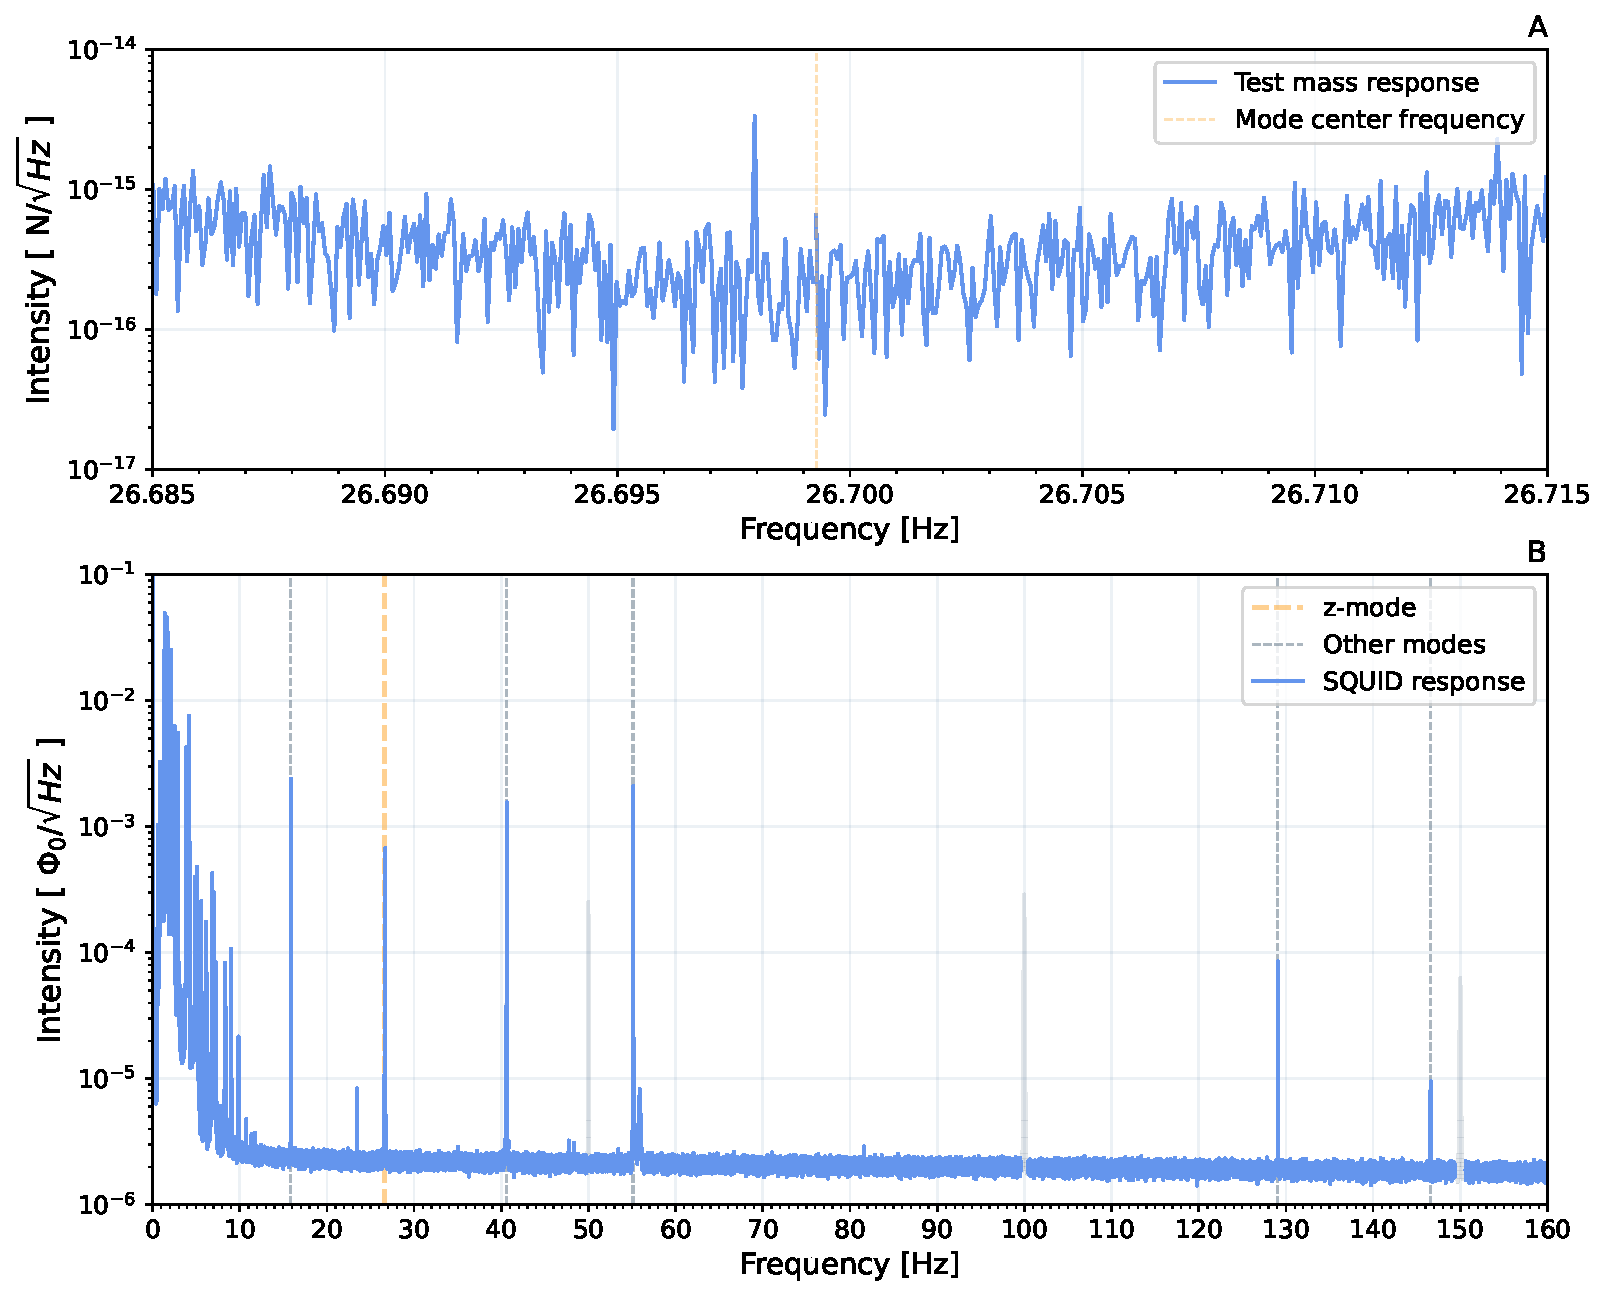
\includegraphics[width=\textwidth]{Results/paper_spectrum_combined.pdf}%, bb=0 0 700 500
\caption{\textbf{\emph{A}}: Force noise of the \SI{27}{Hz} mode when gravitationally driven at \SI{1.3}{mHz} detuning, overnight. \textbf{\emph{B}}: Typical resonator power spectrum. In this figure we have greyed out the regular \SI{50}{Hz} european electrical noise. Which typically has a similar power to the particle resonances.}\label{fig2:spectrum}
\end{figure}

Using this magnetic drive, we determine the decay time of the modes during the subsequent ringdown. For the \SI{26.7}{Hz} mode, we find a lower bound  $\tau = \SI{1.09e5}{s}$, or a Q factor of $Q = \SI{9.13e6}{}$. This procedure is further discussed in appendix~\ref{app:qfactortransfer}. For the other modes, we arrive at Q factors that are about an order of magnitude lower.

We test the force sensitivity of our mode by driving the \SI{26.7}{Hz} mode using the brass masses of the mass-wheel. 
The resulting excitation at one position of the wheel in the force spectrum, is shown in figure~\ref{fig2:spectrum}A. 
The calibration of this spectrum is discussed in appendix~\ref{app:qfactortransfer},~\ref{app:calibration} and~\ref{app:correction_and_conversion}. 
The resulting force noise of this z-mode is approximately $\SI{0.5}{fN/\sqrt{Hz}}$,  or equivalently, a displacement noise of $\SI{60}{pm/\sqrt{Hz}}$, in an \SI{8}{mHz} bandwidth centered around the orange dotted line that indicates the frequency of the resonance. 
Equivalently, we can determine the motion of the trap in which the particle is levitated by dividing the force noise by the spring constant of the confinement potential that keeps the particle around its equilibrium height. 
The spring constant for the z-mode was determined to be k = \SI{12e{-3}}{N/m}, resulting in a trap displacement noise of $\SI{30}{fm/\sqrt{Hz}}$.
This vibrational noise is not yet thermally limited, but rather corresponds to a mode temperature of 3 K, which we attribute to the limits of the vibration isolation inside the cryostat.

In figure~\ref{fig3:force} we show the measured gravitational interaction for different displacements of the wheel, using the method described in appendix~\ref{app:correction_and_conversion}. We also plot the phase of the masses along the wheels rotation for which the particle experiences maximal force, see figure \ref{app:phase}. For the longitudinal displacement, the vertical displacement was held at \SI{48}{} $\pm$ \SI{4}{} centimeter. In the run of vertical positions, the wheel was kept centered with respect to the trap. Included is the expected gravitational signal at the location of the magnetic particle for the z-mode of the particle, which was calculated from an analytical simulation where the mass was taken to consist of multiple point masses. From this same simulation, a systematic error bound was derived, based on an estimated systematic error, for the longitudinal run, of $\pm$5 centimeter longitudinal, $\pm$3 centimeter lateral, and $\pm$4 centimeter vertical, which were estimated from the geometry of the wheel, the mass spring system and the systems used to measure the displacements. For the vertical run, the bounds are $\pm$2 centimeter in each principal direction, based on the increased stability of the system under vertical displacement.

\begin{figure}[ht]%
\centering
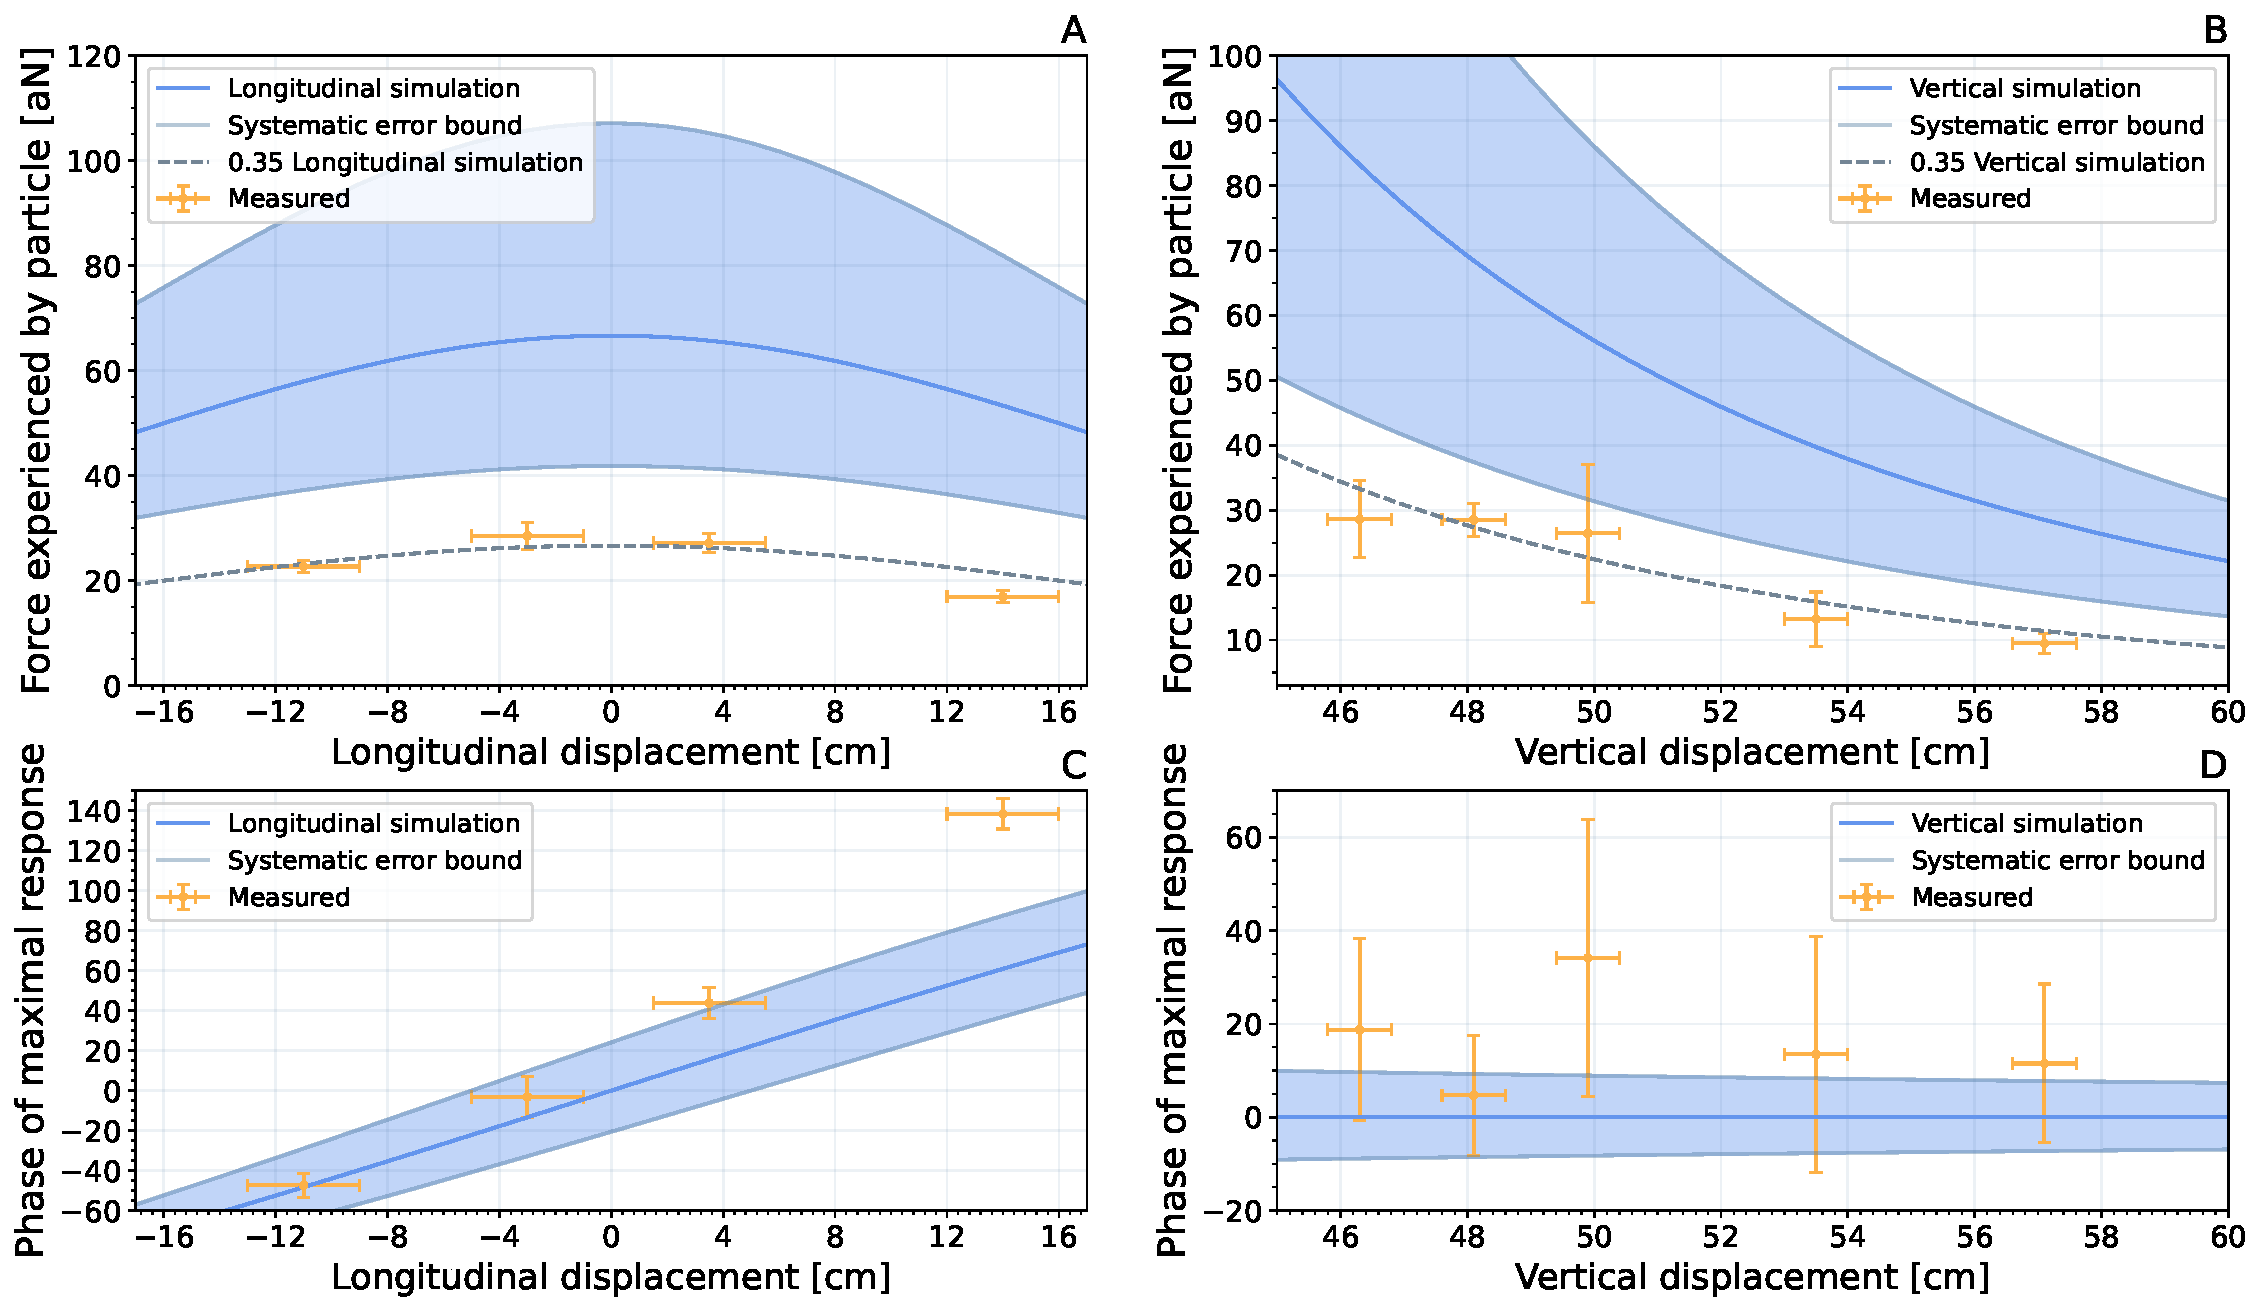
\includegraphics[width=\textwidth]{Results/paper_full_combined.pdf}% , bb=0 0 850 500
\caption{\textbf{\emph{A}}: Force experienced by the mechanical resonator as a result from drive using the mass wheel, for different lateral displacement of the mass wheel relative to the particle. The dashed blue line represents the simulated gravitational force at the position of the magnetic particle as discussed in the main text. The blue area denotes the systematic uncertainty discussed in the text. A second, dashed line is plotted, which has a scaling factor of 0.35 applied, that seems to agree with the data more closely. \textbf{\emph{B}}: Similar to A, but now for a vertical displacement of the mass wheel relative to the particle, when the wheel is kept centered below the particle. Systematic bounds as discussed in the text.   \textbf{\emph{C}}: Here we see the wheel phase at which the magnetic particle experiences the strongest force, plotted against longitudinal displacement. \textbf{\emph{D}}: Similar to C, but now for a vertical displacement.\\
}\label{fig3:force}
\end{figure}

The observed signal agrees with the simulated force signal to within a factor 0.35 with a standard error of 0.02, which was determined by means of an orthogonal distance regression fit to the data.

We attribute this constant factor to the effect of the wheel on the trap. Since the centre of mass of the particle and the trap together with the holder are closely spaced, they all experience a similar gravitational gradient. For the trap, however, the frequency of the gravitational drive is far above resonance (that is: the resonance determined by the suspension of the trap and holder by springs in the form of the mass spring system), which naturally gives rise to a 180\textdegree\ phase shift in the trap's response. This phase shift means that the resulting motion of the trap leads to a suppression of the particle response.






